\chapter{Introduction}\label{ch:intro}

In this thesis, I explore certain aspects of the so-called high-temperature superconductors. While these materials were discovered fairly recently (1986), they have a rich history with hundreds of thousands of citations and, to this day, a lively debate surrounding the microscopic nature of this mysterious macroscopic quantum state. The purpose of this chapter is to briefly state the `the story so far' in broad strokes, and then dive deeper into state-of-the-art research relevant for the work performed in this thesis.

\section{Superconductivity}
Superconductivity is a state of matter where a material is able to conduct electricity with \emph{zero} DC resistance below a certain critical temperature $T_\text{c}$. Since we, fortunately, live in a world where the `spherical cow in a vacuum' model is a very crude approximation to reality, it is remarkable to find \emph{real} materials where electrons can propagate without friction. In fact, experiments have shown, that under the right conditions it is possible to keep a persistent superconducting current running for 100000 years \cite{File1963}!

Superconductivity was first discovered in 1911 by Kamerlingh Onnes, essentially as a consequence of being able to liquefy helium in 1908 and reach temperatures close to absolute zero (see \cite{VanDelft2010} and references therein for a breakdown of the experiments). His low-temperature measurement of lead revealed a sudden drop in resistivity at \SI{4.2}{\kelvin}, as seen in the historic plot on figure \ref{fig:onnes}

\begin{figure}
    \centering
    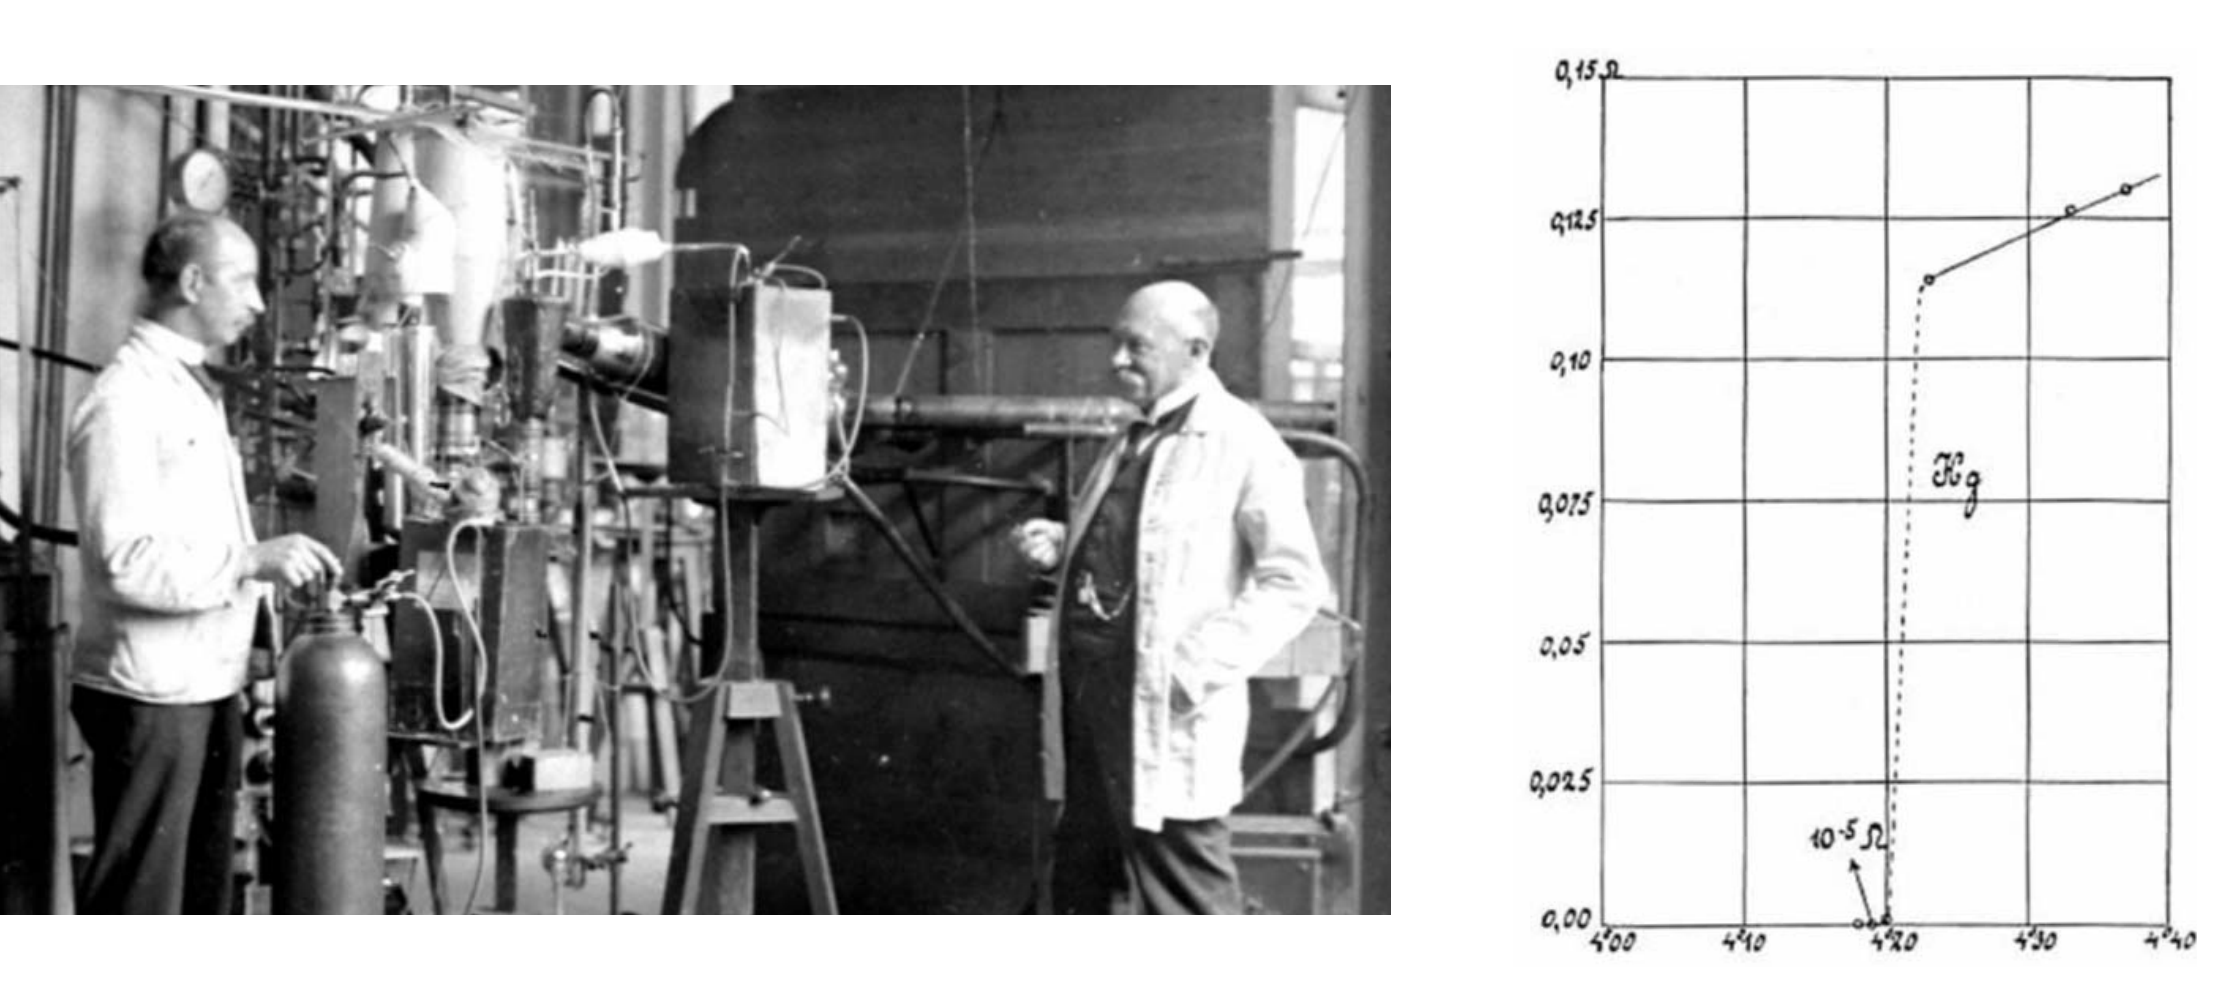
\includegraphics[width=\textwidth]{fig/intro/onnes.png}
    \caption[SC of elemental lead]{\textbf{Left}: Kammerling Onnes (right) and his chief engineer (left) in their cryogenics lab. \textbf{Right}: Resistivity as a function of temperature in elemental Lead. Both images from \cite{VanDelft2010}.}
    \label{fig:onnes}
\end{figure}

\begin{figure}
    \centering
    \missingfigure{Meissner effect}
    \caption[Meissner effect]{Meissner effect}
    \label{fig:meissner}
\end{figure}

Despite this remarkable experimental result, it would be 20 years for the next major milestone to appear. In 1933 the Meissner effect was discovered \cite{Meissner1933}, showing that superconducting materials would completely resist applied magnetic field by exhibiting perfect diamagnetism as sketched in figure \ref{fig:meissner}. In 1935 this effect was phenomenologically explained by the London equations, showing that the Meissner effect is due to superconducting currents on the surface of the material \cite{London1935}. From their relatively simple set of equations, an observable length scale known as the penetration depth was defined
%
\[ \lambda_\text{L} = \sqrt{\frac{m}{\mu_0 n q^2}} \, \]
%
where $\mu_0$ is the permeability of free space, $n$ the number concentration of the superconducting carriers, $m$ the electron mass and $q$ the electron charge. This length scale determines how an external magnetic field penetrates the superconductor through the relationship $B(x) = B(0) \exp (-x / \lambda)$. $\lambda$ is typically on the order of \SIrange{20}{100}{\nano\meter} \cite{Kittel2005}.

Another roughly 20 years would pass until Landau's work on phase transitions paved the way to understanding the superconducting phase transition as a thermodynamic quantity through the Ginzburg-Landau equations in 1950 \cite{Ginzburg2009}. I will not repeat the details here, but the idea is to make a polynomial expansion of the free energy as a function of a complex superconducting wavefunction $\psi$. As the material is cooled below $T_\text{c}$, $\psi$ `choses' a phase and breaks gauge symmetry, analogous to how a ferromagnet choses a common direction for the magnetic moment at the magnetic phase transition. This description predicts an new characteristic length scale of the superconductor called the \emph{coherence length} $\xi$ and recasts the penetration depth in terms of $\psi$:
%
\[ \xi = \sqrt{\frac{\hbar^2}{4m|\alpha|}} \qquad \lambda = \sqrt{\frac{m}{4\mu_0 e^2 \psi_0^2 }} \, , \]
%
where $\alpha$ is a phenomenological parameter of the polynomial expansion. The ratio of these parameters, $\kappa = \lambda / \xi$, are used to classify superconductors into type-I ($\kappa < 1 / \sqrt{2}$) and type-II ($\kappa > 1 / \sqrt{2}$). The significance of $\kappa > 1 / \sqrt{2}$ can be understood as a threshold where the surface tension between normal and superconducting phases becomes negative \cite{Abrikosov1957}. Intuitively, the coherence length $\xi$ defines the shortest length within which the superconducting carrier concentration are allowed to change considerably. For elemental metals $\xi$ can be on the nanometre to micrometre scale: \SI{1600}{\nano\meter} in Al and \SI{83}{\nano\meter} in Pb \cite{Kittel2005}. In the cuprates (which will be discussed in detail in the next section), $\xi$ is typically on the order of a few lattice spacings (\SI{1}{\nano\meter} in YBa$_2$Cu$_3$O$_{7-\delta}$ \cite{Tomimoto1999}).

Based on Ginzburg-Landau theory, \citeauthor{Abrikosov1957} predicted the existence of vortices in Type-II superconductors, which showed excellent agreement with the measured magnetization of several lead alloys \cite{Abrikosov1957}. These vortices can be pinned by defects and form a lattice that we have been able to image using modern day microscopy techniques (see e.g. \cite{Wells2015} for a recent example with beautiful real-space images). The experimental evidence piled up \cite{Doll1961, Deaver1961}, and it quickly became evident that Ginzburg-Landau theory is applicable to most known superconductors, including the cuprates and iron-based varieties.

Despite the descriptive power of Ginzburg-Landau theory, we are left with no recipe on how to construct, even theoretically, `better' superconductors. In order to manipulate material properties, it is necessary to understand the microscopic properties that lead to macroscopic behaviour (e.g. how phonons influence thermal properties or how magnetic exchange influence magnetic properties. Inspired by Ginzburg-Landau theory, rapid progress towards a microscopic theory was being made in the mid 1950s, culminating in the famous BCS theory formulated by Bardeen, Cooper and Schrieffer \cite{Bardeen1957}. 

BCS theory is based on the assumption that an attractive interaction between electrons at the Fermi level can result in so-called `cooper-pairs', a bosonic quasi-particle consisting of an electron pair of opposite momentum and spin. The bosonic nature of this quasi-particle can, at low temperatures, result in a Bose-Einstein condensate where a large fraction of these electron pairs occupy the lowest energy quantum state. This microscopic theory of superconductivity made several testable predictions, such as the appearance of an energy gap with a temperature-dependent width $\Delta(T)$ in the electronic density of states related to the critical temperature through the relationship
%
\[ 2\Delta(T=0) = 3.5 k_\text{B} T_\text{c} \, , \]
%
where $k_\text{B}$ is the Boltzmann constant. A few years later electron tunnelling experiments confirmed this prediction with reasonable accuracy \cite{Giaever1960, Giaever1960a}. Additionally, \citeauthor{Josephson1962} predicted that superconducting currents could tunnel across an insulating a barrier \cite{Josephson1962}, experimentally verified a few years later \cite{Jaklevic1965}.

While BCS theory predicts an attractive interaction between electrons, the original paper \cite{Bardeen1957} makes no assumption about the nature of this interaction. Some experiments, performed a few years prior, showed that $T_\text{c}$ of Hg$^{198}$ was higher when compared to that of natural Hg (avg. atomic weight of 200.6) \cite{Maxwell1950, Reynolds1950}. Since the chemistry of these materials can be assumed identical, this experiment suggests a positive correlation between phonon frequencies and $T_\text{c}$, since lighter elements have more energetic vibrations. Assuming an attractive potential due to lattice vibrations, BCS theory could relate the attractive interaction to phonon frequencies and predict a relative relationship between isotopic mass and critical temperature \cite{DeLaunay1954}:
%
\[ T_\text{c} \propto \frac{1}{\sqrt{m_\text{ion}}} \, , \]
%
where $m_\text{ion}$ is the isotopic mass of the constituent ionic species. With BCS theory, superconductivity in many elemental metals were believed to be `solved' with the identification of phonon-mediated superconductivity. Unfortunately, this discovery also set a \emph{practical} upper limit on $T_\text{c}$. In order to increase phonon frequencies, and thus critical temperatures, we need materials with low mass atomic species, while still being crystalline. At ambient pressure this practical upper limit is often quoted to be around \SI{30}{\kelvin}. A good demonstration of this principle is actually a counter-example where researchers were able to reach a critical temperature of $T_\text{c} = \SI{200}{\kelvin}$ by applying a pressure of \SI{155}{\giga\pascal} to H$_2$S \cite{Drozdov2015}. This material contains the light atomic species we require, but cannot crystallize at ambient pressures so we can only reach high critical temperatures under extreme conditions. A different example is the highly unusual case of MgB$_2$, where coincidences add up to an unusually high electron-phonon coupling resulting in a critical temperature of $T_\text{c} = \SI{39}{\kelvin}$ \cite{Nagamatsu2001}.

While this thesis concerns cuprates which are not simple described as BCS superconductors and, in principle, the thesis could have been written without ever mentioning them, I believe that the history of conventional superconductivity emphasises exactly what is desired from a `solution' to high-temperature superconductivity. It is also a fascinating story due to the fact that the tools to solve the problem were not even close to being developed when the phenomenon was discovered. It took roughly 50 years for a satisfying conclusion and we have only been working on the cuprates for roughly 30 years. 

\section{Cuprates}
With this brief introduction to superconductivity, I will proceed with an introduction to cuprate superconductivity. While the previous section contains research results and explanations generally accepted and agreed upon, it is difficult to capture an unbiased view of cuprate research. As such, the following will be somewhat narrowly focused. While this is a reasonable choice for this introduction, it is important to realize just how massive the field is and how impossible it is to know every last detail. That being said, I have thoroughly enjoyed exploring the vast literature and I will recommend anyone reading this to do the same.

Before we begin, I want to establish some of the nomenclature  As the title of this thesis suggest, I am working on the so-called `high-temperature superconductors'. This definition essentially only concerns itself with the value of the critical temperature (usually above the `BCS-limit' of \SI{30}{\kelvin}), without saying anything about other physical properties. On the other hand Type-I and Type-II, as seen in the previous section, are rigidly defined with respect to their properties as defined through Ginzburg-Landau Theory. Finally, `conventional superconductors' are those that can be microscopically described with BCS theory, while 'unconventional superconductors' cannot. While cuprates are relatively simple crystals, most of them have a variety of names and abbreviations attached to them. Table \ref{tab:cuprates} lists the most important ones along with their critical temperatures and a few other physical properties.

\begin{table}
    \caption[table of cuprates]{list of cuprates}
    \label{tab:cuprates}
    \missingfigure{Table of cuprates, formulae, names, Tc, crystal structure}
\end{table}

\subsection{The discovery of LBCO}
Roughly 30 years after BSC theory, in 1986, Bednorz and M\"uller discovered a new type of superconductor while trying to manipulate the electronic properties of the anti-ferromagnetic insulator La$_2$CuO$_4$. By effectively removing a small number of electrons from the system by substitution of dopant species, they achieved a record $T_\text{c}$ of \SI{30}{\kelvin}. Shortly after, in 1987, the sister-compound YBa$_2$Cu$_3$O$_{7-\delta}$ was discovered, shattering previous records and finally achieving a critical temperature $T_\text{c} = \SI{93}{\kelvin}$ that could be reached using liquid nitrogen \cite{Wu1987}.

While the increased critical temperatures are remarkable on their own, it quickly became apparent that we were dealing with a completely new type of superconductivity which cannot be explained with BCS theory. The normal state ($T > T_\text{c}$) of cuprate superconductors is as, if not more, complex when compared to the superconducting state and the BCS assumption of being metallic in the normal state is generally not fulfilled. In addition, the BCS relationship between isotopic mass critical temperature ($T_\text{c} \propto m_\text{ion}^{-0.5}$) is not fulfilled when performing O$^{16}$/O$^{18}$ isotopic substitution \cite{Suryadijaya2005}.

Similar to semiconductors, the properties of the cuprates are dramatically changed with the introduction of dopant species. In general, we call the addition of electrons \emph{electron doping} and the removal of electrons \emph{hole doping}. In the original paper, La$_2$CuO$_4$ was hole-doped by exchanging La$^{3+}$ with Ba$^{2+}$. We define the amount of hole-doping ($n_\text{h}$) as the fraction of substituted atomic species per CuO$_2$ layer. The amount of electron doping ($n_\text{e}$) is defined similarly. In general, the undoped compounds $n_\text{h} = 0$ are antiferromagnetic insulators and you need a small amount of doping to make the materials superconducting. It it also possible to dope too much (typically $n_\text{h} > 0.25$) and the materials become non-superconducting metals. 

The fact that we need finite amounts of doping in order to make cuprates superconducting, makes them inherently inhomogeneous materials. This inhomogeneity may or may not be important for cuprate superconductivity, but there is no denying that it exists. In fact, recent STM studies on Bi$_2$Sr$_2$CaCu$_2$O$_{8+\delta}$ have shown significant spatial inhomogeneities due to random distributions of defects \cite{Ruan2018}. %If this inhomogeneity is relevant, it presents us with a great difficulty in producing models that can explain superconductivity; adding too much complexity can be detrimental to explanatory power.

\subsection{Structure}
Cuprate superconductors are characterized by a layered structure where CuO$_2$ layers are separated by so-called charge reservoirs (or spacer layers). In general, the conventional Bravais lattice is either tetragonal or orthorhombic with the CuO$_2$ layers in the $a$-$b$ plane. A few examples of cuprate crystal structures is shown in figure \ref{fig:cuprate_family_structures}. The different structures are generally characterized by the number $n$ of subsequent CuO$_2$ layers. Interestingly, increasing $n$ generally improves the critical temperature $T_\text{c}$ up to $n = 3$. It has been suggested that the decrease at $n \geq 3$ could be due to the fact that the `inner' and `outer' CuO$_2$ layers cannot reach similar doping \cite{Wesche2017}.

\begin{figure}
    \centering
    \missingfigure{selection of cuprate crystal structures, LSCO on the left}
    \caption[various cuprate structures]{various cuprate structures}
    \label{fig:cuprate_family_structures}
\end{figure}

Doping is performed either by substitution or addition of dopant species as indicated by figure \ref{fig:cuprate_family_structures}. Doping thus necessarily changes the lattice either due to a difference in ionic radii of a substitutional dopant or a strain in the lattice because of an interstitial species. In the case of substitutional doping of La$_2$CuO$_4$, the structural and electronic properties vary wildly (as we shall see in section \ref{sec:lsco}) depending on the dopant species (Ba, Sr).

Different members of the cuprate family have their own structural peculiarities. In single-layer LSCO, many structural properties are linked to the CuO$_6$ octahedra which are not present in structures with $n \geq 2$ and In YBCO, Cu-O chains form along the crystallographic $b$-axis. Despite these specific structural properties of the various cuprates, they are all equipped with square CuO$_2$ planes and have remarkably similar (electronic) phase diagrams.

\subsection{Phase diagram}
A general phase diagram for the cuprates is shown in figure \ref{fig:cuprate_phase_keimer} illustrating the many macroscopic and microscopic phases in the cuprates as a function of temperature and doping. First, figure \ref{fig:cuprate_phase_keimer} (left) shows an unexpected asymmetry between hole and electron-doping. Since cuprates are superconducting for a wider range of doping on the hole-doped side, most research focuses on this side of the phase diagram\todo{Other arguments? More discussion of the assymetry?}. Second, as shown in figure \ref{fig:cuprate_phase_keimer} (right), cuprates are only superconducting for a narrow range of hole doping typically between $n_h = 0.05$ and $n_h = 0.25$ with a maximum around $n_h = 0.15$. This region is known as the `superconducting dome'. 

\begin{figure}
    \centering
    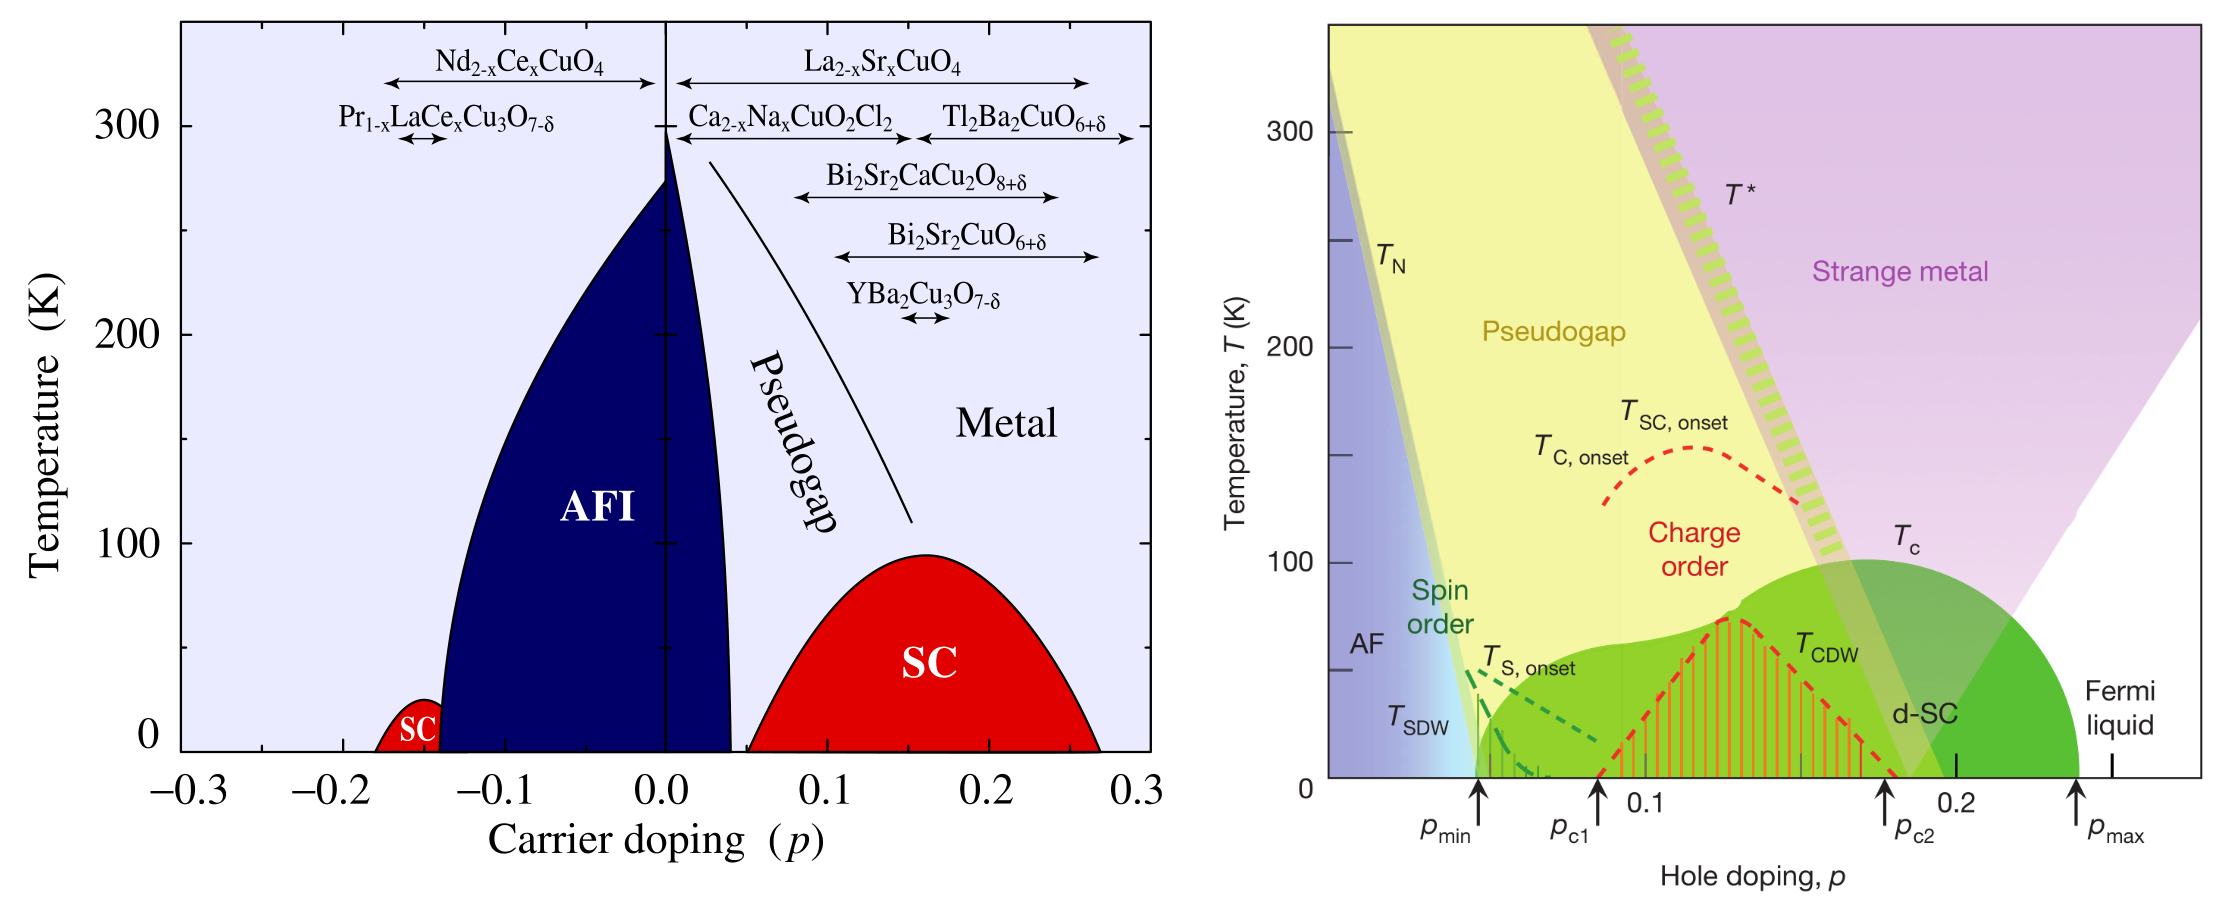
\includegraphics[width=\textwidth]{fig/intro/keimer.png}
    \caption[cuprate phase diagrams]{\textbf{Left:} Generalized phase cuprate phase diagram for selected electron- and hole-doped materials, emphasizing the asymmetry between the two sides of the phase diagram. From \cite{Peets2007}. \textbf{Right:} Generalized phase diagram for the hole-doped side annotated with microscopic ordering phenomena. From \cite{Keimer2015}.}
    \label{fig:cuprate_phase_keimer}
\end{figure}

I emphasize here the very different states of matter at the boundaries of the superconducting dome at $T=0$: Over-doped cuprates are typically metals while underdoped cuprates are magnetic insulators. In some sense, superconductivity is optimized in a region between localized (magnet) and itinerant (metal) behaviour -- a region also containing poorly understood normal state ($T > T_\text{c}$) behaviour such as the Pseudogap and strange metal phase.

The Pseudogap is a curious phenomena first observed in NMR measurements of YBCO \cite{Alloul1989} and later on in the $c$-axis resistivity \cite{Homes1993} and specific heat \cite{Loram1993}. The name comes from the fact that, by now, it is generally associated with the opening of a gap in the electronic density of states (see below). The difficulty in finding a microscopic origin of the phase transition at the Pseudogap temperature $T^*$ has attracted as much attention as the superconducting transition itself. Many researchers believe that the key to understanding the superconducting transition is directly related to the Pseudogap. One idea is that of `pre-formed pairs', where Cooper pairs start forming at $T^*$, but the macroscopic superconducting state fails to settle between $T^*$ and $T_\text{c}$ due to incoherent fluctuations in the phase of the pairing field ($\psi$ in Ginzburg-Landau theory) \cite{Emery1995, Curty2003}.\todo{maybe remove this last bit, too technical}

The strange metal phase is possibly the least understood part of the cuprate phase diagram \cite{Keimer2015}. A `strange' metal is essentially a phase of matter where the theory of `normal' metals (Fermi liquids) breaks down and is a phenomenon seen in a number of correlated electron systems, not just the cuprates. A significant indicator of this behaviour is a linear temperature-dependence of resistivity (see e.g. \cite{Martin1990} for a cuprate example), where a normal Fermi liquid varies as $T^2$ at low temperatures. A recent study even suggests that this linear-in-$T$ resistivity in the cuprates is a generic property related to a universal scattering rate \cite{Legros2018}.

By outlining the the phase diagram in this way, I intend to illustrate both the difficulty of solving the cuprate problem and the many experimental methods and theoretical tools necessary to investigate the various features of this complex phase diagram. Until now, apart from crystallographic information, we have mainly considered \emph{macroscopic} behaviour through bulk measurements such as resistivity, specific heat, optical band gap or magnetic susceptibility. We now turn to a brief overview of \emph{microscopic} behaviour, starting with momentum-resolved measurements of the Fermi surface.

\subsection{Fermi Surface}
Angle-Resolved Photoemission Spectroscopy (ARPES) is a method in X-ray spectroscopy that directly probes the electronic band structure of materials. This method has been extremely important in strongly correlated electron systems in general and has a rich history with the cuprates (see the extensive review by \citeauthor{Damascelli2003} \cite{Damascelli2003}, which also serves as a good introduction to the experimental method). Allthough a few ARPES experiments were carried out during my phd project (see \ref{sec:}) this thesis primarily concerns itself with neutron scattering as an experimental technique. Thus the technical details of ARPES will not be reviewed here but can be found in literature (\cite{Osterwalder2014} is a great introduction).

ARPES experiments are extremely surface sensitive experiments with a typical penetration depth of a few lattice spacings, and thus requires samples that cleave naturally at the interface one wants to probe. While cuprates have a layered structure, the materials themselves are also quite brittle, so the in-situ cleaving procedure can be challenging. However, since superconductivity is generally associated with a gap at the Fermi level due to Cooper pair formation, this technique is extremely valuable for our understanding of unconventional superconductivity.

\begin{figure}
    \centering
    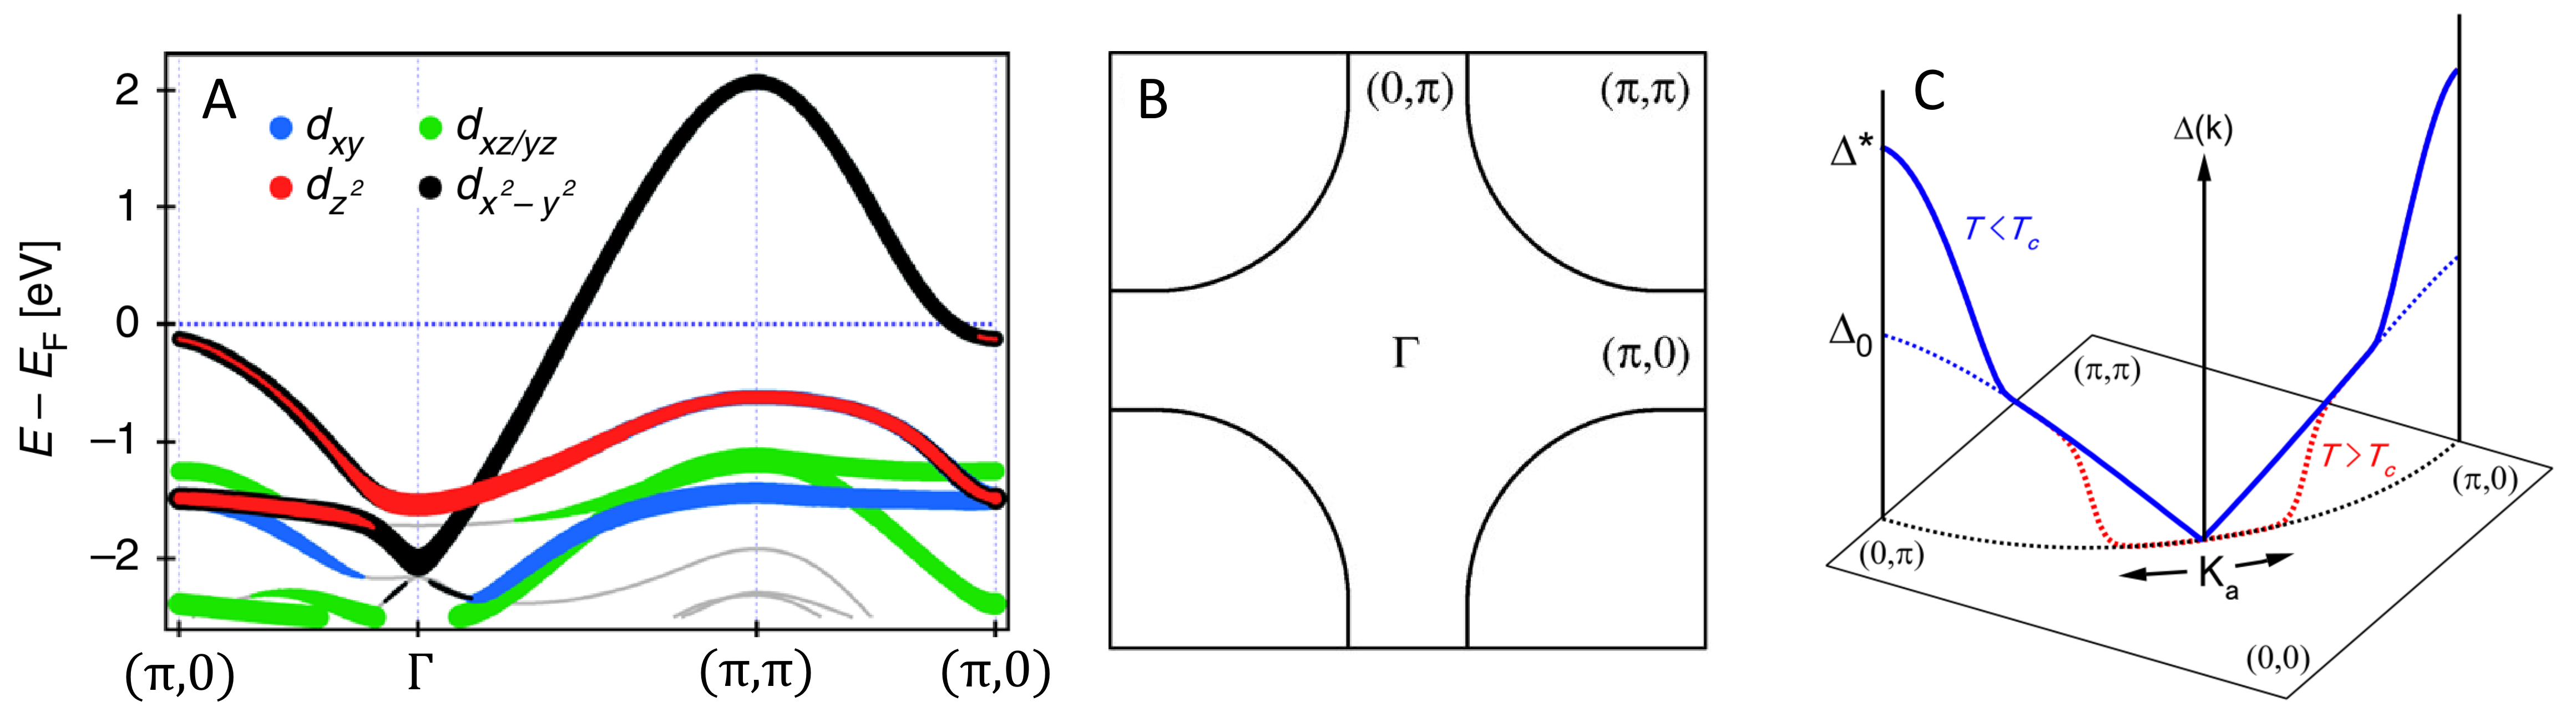
\includegraphics[width=\textwidth]{fig/intro/arpes_fermisurface.png}
    \caption[ARPES fermi surface schematic]{ARPES fermi surface schematic DFT from \cite{Matt2018}, metal schematic from \cite{Damascelli2003}, Gap structure from \cite{Yoshida2011}}
    \label{fig:intro_arpes}
\end{figure}

Figure \ref{fig:intro_arpes}A and figure \ref{fig:intro_arpes}B shows our `reference' Fermi surface as calculated from Density Functional Theory (more on this in chapter \ref{ch:method}), representing the overdoped part of the phase diagram. Here we see that the conduction band is made up of electrons from the $d_{x^2-y^2}$ orbital that cross the Fermi level halfway towards the antiferromagnetic wave vector $(\pi,\pi)$. This crossing defines the so-called `Fermi arcs' shown in figure \ref{fig:intro_arpes}B. As we move towards the optimally underdoped or optimally doped part of the phase diagram, the Fermi arcs are broken up as shown in figure \ref{fig:intro_arpes}C, revealing both the superconducting gap $\Delta_0$ and the pseudogap $\Delta^*$. These gaps have been identified and distinguished in experiments on Bi2212 as shown in figure \ref{fig:intro_arpes_feng}. These discontinuities at the Fermi surface is also a direct experimental evidence that we are dealing with a system that cannot be explained by conventional one-electron theories.

\begin{figure}[]
    \centering
    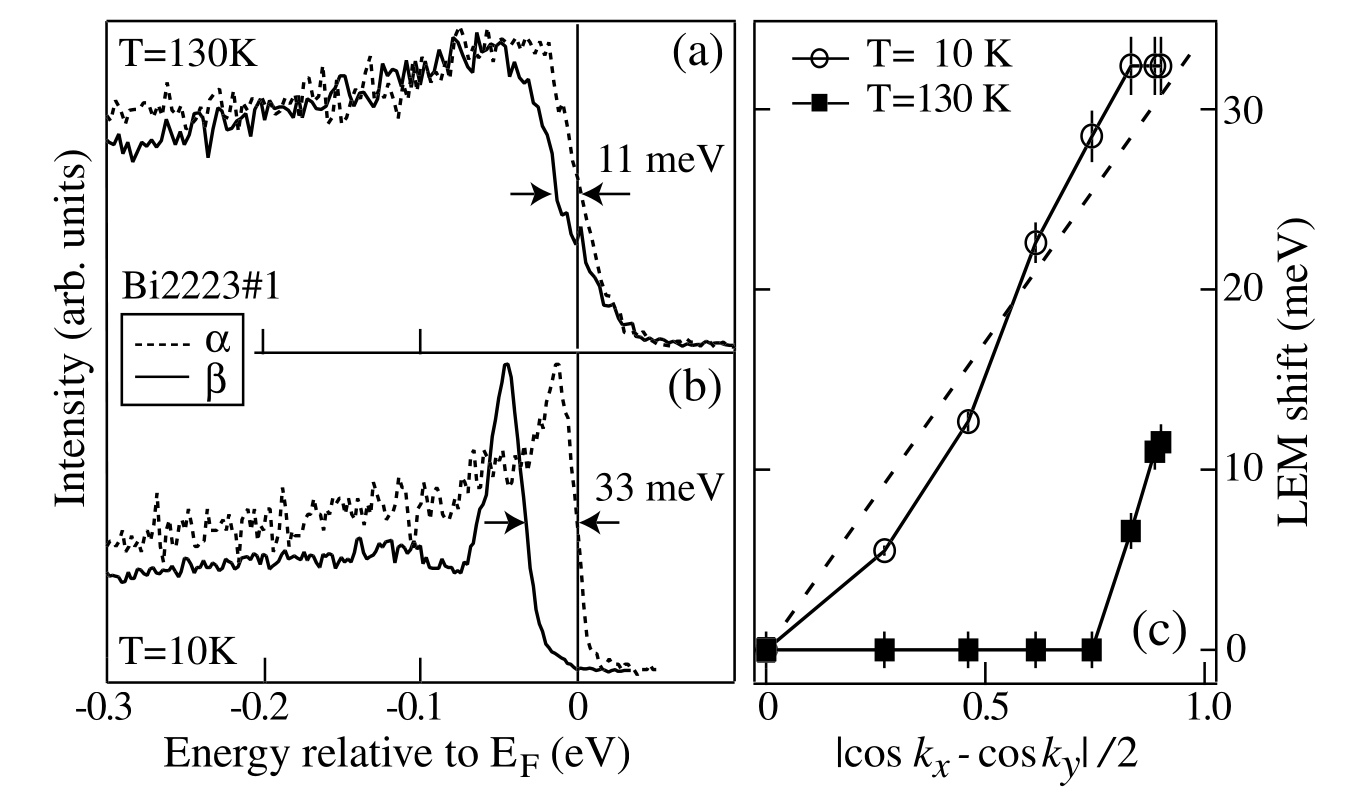
\includegraphics[width=0.7\textwidth]{fig/intro/arpes_feng.png}
    \caption[ARPES gaps data]{ARPES gaps data from \cite{Feng2002}}
    \label{fig:intro_arpes_feng}
\end{figure}

The structure of this superconducting gap ($\Delta_0$) reveals certain symmetries of which, in turn, reveals the `pairing symmetry' of the Cooper pairs (see \cite{Tsuei2000} for a review) which is related to their total spin and orbital angular momentum. These symmetries are what gives rise to the naming scheme taken from electron orbitals, where $s$-wave superconductors have an isotropic gap and $d$-wave superconductors have a gap with the functional form $\Delta^* = | \cos k_x - \cos k_y | / 2$, where $(k_x, k_y)$ are wave vectors along the Fermi arcs (see $\Delta_0$ in figure \ref{fig:intro_arpes}C). Other symmetries have also been found, such as $p$-wave in Sr$_2$RuO$_4$ \cite{Mackenzie2003} and $f$-wave in UPt$_3$ \cite{Joynt2002}.

These observations of the electronic band structure and Fermi surface thus tells us a lot about the nature of the superconducting pairing, it does not directly give us a \emph{mechanism} for the pairing similar to how BCS theory and the isotope effect gave us Cooper pairs due to phonons. While theoreticians have been working tirelessly to construct models that can explain all these behaviours, no consensus have been reached at this point. For this reason, some experimentalists are looking at microscopic correlations in order to uncover what the atoms and electrons are `doing' at the various phase transitions summarized in figure \ref{fig:cuprate_phase_keimer}.

\subsection{Microscopic correlations}
When any type of phase transition happens in a material it, by definition, must be caused by a microscopic phenomenon. Any satisfactory theory in condensed matter physics should be able to explain macroscopic behaviour starting from the constituent parts and experiment that can probe microscopic behaviour are often essential. Sometimes, as with the isotope effect in conventional superconductors, we can infer the microscopic behaviour in indirect ways, but often it is necessary to probe the atomic length scales directly. The microscopic probe used in this thesis is neutron scattering, which is used to infer structure and dynamics through a scattering process between a beam of neutrons and a sample. Technical details of the method will be covered in chapter \ref{ch:method}, but for now we briefly state some of the important results.

As mentioned earlier, the undoped cuprates are antiferromagnetic insulators. While an odd number of electrons in the system usually results in metallic behaviour, the localized shape of the $d$ orbitals results in static magnetism due to an exchange interaction $J$ and the physics are reasonably well-described within linear spin wave theory \cite{Headings2010}.

As one moves to finite values of hole doping, this antiferromagnetic order is interrupted and some electrons can start to propagate through the material. A common analogy is that of magnetic interactions causing a traffic jam of electrons that is then relieved as one moves from left to right in the phase diagram (figure \ref{fig:cuprate_phase_keimer}). A real-space visualization of this analogy is shown in figure \ref{fig:electron_traffic_jam}. It turns out that this gradual destruction of magnetic order happens in a peculiar way where the magnetism becomes incommensurate with an incommensurability $\delta$ that is linear in doping as shown in figure \ref{fig:yamada_plot}A.

\begin{figure}
    \centering
    \missingfigure{electron traffic jam}
    \caption[electron traffic jam analogy]{electron traffic jam analogy}
    \label{fig:electron_traffic_jam}
\end{figure}

\begin{figure}
    \centering
    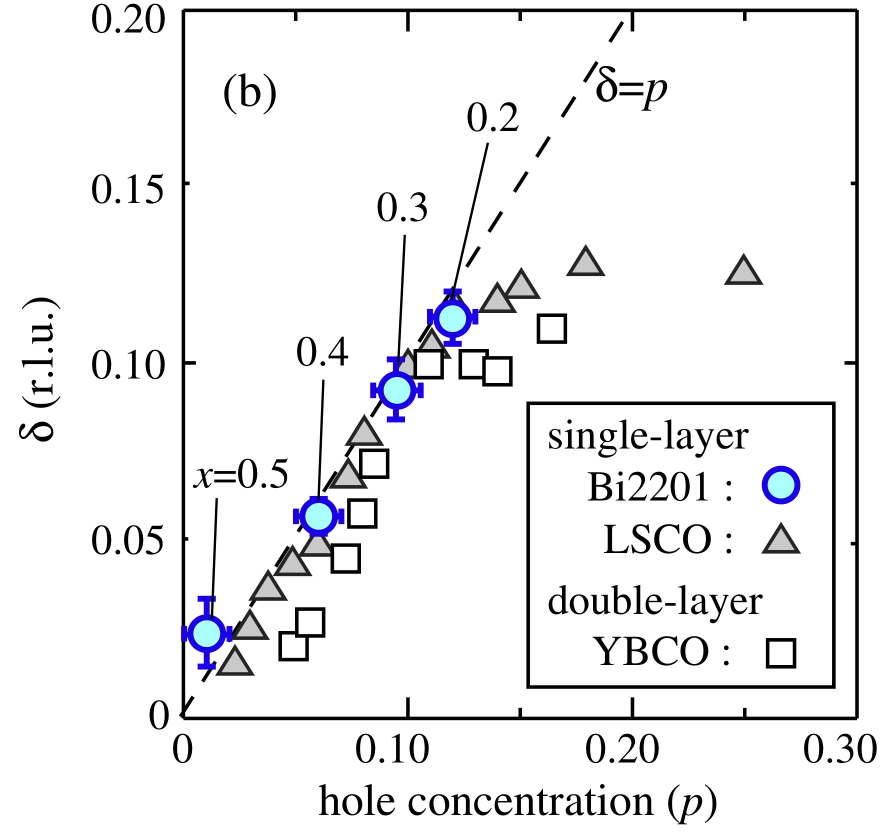
\includegraphics[width=0.49\textwidth]{fig/intro/enoki_plot.png}
    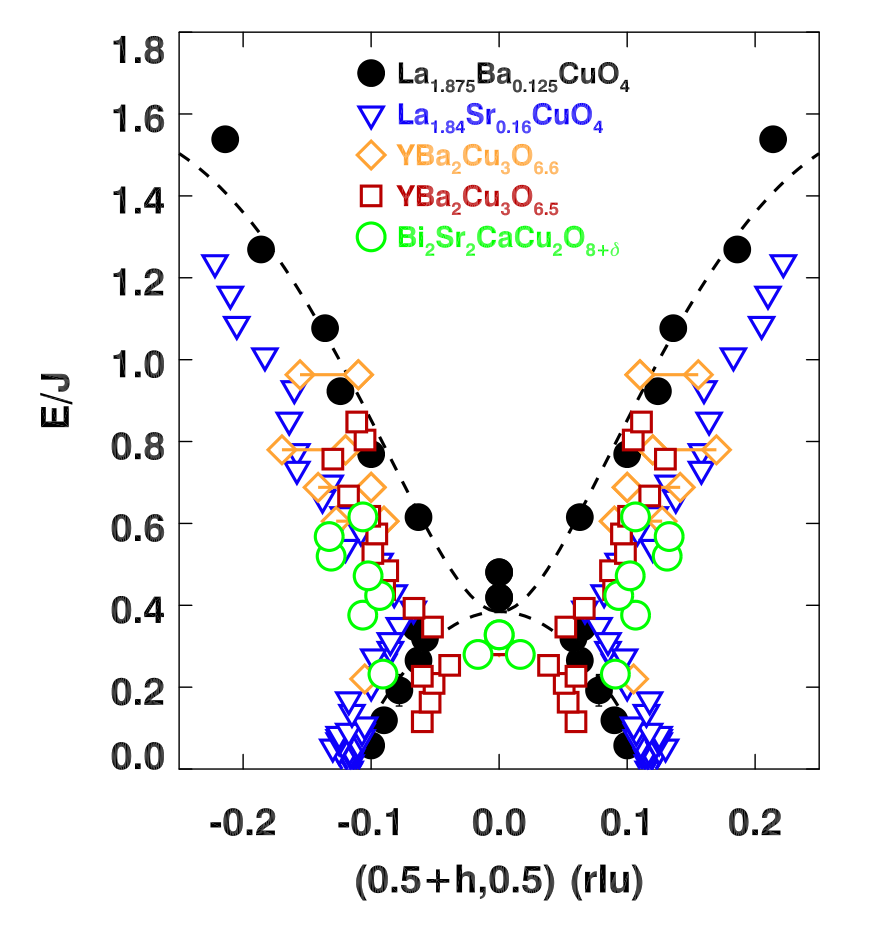
\includegraphics[width=0.49\textwidth]{fig/intro/hourglass.png}
    \caption[yamada plot plus hourglass]{yamada plot plus hourglass}
    \label{fig:yamada_plot}
\end{figure}

Figure \ref{fig:yamada_plot}A also reveals a saturation of this incommensurability at $x \approx \frac{1}{8}$, suggesting that period-8 magnetic order is somehow important for cuprate superconductivity. On the other hand, the phase diagram reveals that $T_\text{c}$ is supressed at exactly this doping in a number of compounds, with optimal $T_\text{c}$ requiring a few percent more doped holes per CuO$_2$ plane at $n_\text{h} \approx 0.16$. It thus appears as if these observations are universal for the cuprates but at the same time detrimental for superconductivity. This `$\frac{1}{8}$ conundrum' has given rise to the concept of competing orders\todo{reference}, where superconductivity emerges near a plethora of near-degenerate electronic phases where some of them are detrimental to superconductivity.

The excitations of this magnetic order also reveals a universality as shown in figure \ref{fig:yamada_plot}B. It turns out that the magnetic fluctuations from this incommensurate order has a highly unusual `hourglass'-shape, where the `neck' of the hourglass is scaled by the strength of the magnetic exchange in the parent compound. Additionally, when static magnetic order disappears the fluctuations persist and become gapped. Details of this behaviour will be outlined below in the case of LSCO.

These observations, together with the $d$-wave structure of the Fermi surface, intuitively points to a picture where this dual behaviour of the $d_{x^2-y^2}$ electrons is the key to understanding cuprate superconductivity. One popular approach is one where pairing happens not due to an external attractive potential, but through spin fluctuations of the electrons themselves \cite{Scalapino2012}. While these models are not without their problems (\citeauthor{Anderson2007} has argued that the idea of a bosonic glue might not even be appropriate \cite{Anderson2007}), they reproduce parts of the phase diagram quite well\todo{reference}.

\section{La214 and stripe order}\label{sec:lsco}
I will now depart from universal observations in the cuprates and focus on a particular class of cuprates based on the parent compound La$_2$CuO$_4$ (see figure \ref{fig:cuprate_family_structures}). Sometimes known as `La214' or with specific acronyms depending on the dopant species, these materials are single-layer cuprates with a relatively simple crystal structure and a maximum critical temperature $T_\text{c} \approx \SI{40}{\kelvin}$.

Since this thesis is focussed on specific structural aspects and phonon dynamics, this `relatively' simple crystal structure is a particularly strong point for us. Since we want to model the full 3-dimensional structure using computationally heavy simulation methods, it is advantageous to consider the simplest system possible. In addition, since the lanthanum cuprates were the first so-called 'high-temperature superconductors` to be discovered, there is a massive amount of literature on which to build our ideas from.

La$_2$CuO$_4$ can be doped by substitution of La with various atomic species where some of them results in hole doping (e.g. Ba, Sr), while others have been used to modify the structure without changing the effective hole doping (e.g. Nd, Eu). Table \ref{tab:dopants} shows the ionic radius and oxidation state (which determines hole doping) of the species that can be used to dope La$_2$CuO$_4$.

\begin{table}
    \caption{table of dopants \cite{Hucker2012}}
    \label{tab:dopants}
    \missingfigure{table of dopants}
\end{table}

It turns out that La214 cuprates have particularly pronounced physics with regards to behaviour at $n_\text{h} = \frac{1}{8}$. In LBCO, superconductivity is almost completely supressed at $n_\text{h} = \frac{1}{8}$, while in LSCO we only see a small plateau. In fact, by performing a combination of substitutions it is possible to create materials such as LNSCO where superconductivity is completely supressed while being at an otherwise `optimal' doping level. A common thread for LBCO and LNSCO is that this suppression of $T_\text{c}$ happens simultaneously with a tetragonal structural phase. I note here that a tetragonal phase in itself does not inherently prohibit superconductivity since LSCO is tetragonal at low temperatures for $n_\text{h} \geq 0.2125$ \cite{Radaelli1994a}. We thus appear to be in a situation where crystal symmetry has a non-trivial relationship with superconductivity. For a thorough discussion of this particular topic, see the review by \citeauthor{Hucker2012} \cite{Hucker2012}.

It can thus be argued that La214 cuprates are the appropriate materials in which to examine the significance of the $n_\text{h} = \frac{1}{8}$ phase and a lot of attention was given to these phenomena in the early 1990s, culminating in the discovery of so-called `stripe order' in non-superconducting LNSCO \cite{Tranquada1995}. The stripe model is one where the magnetic period-8 order appears simultaneously with a period-4 charge order. These observations led to the stripe model as shown in figure \ref{fig:stripe_model_hucker}, where the magnetic order is separated by one-dimensional `stripes' of charge. 

\begin{figure}
    \centering
    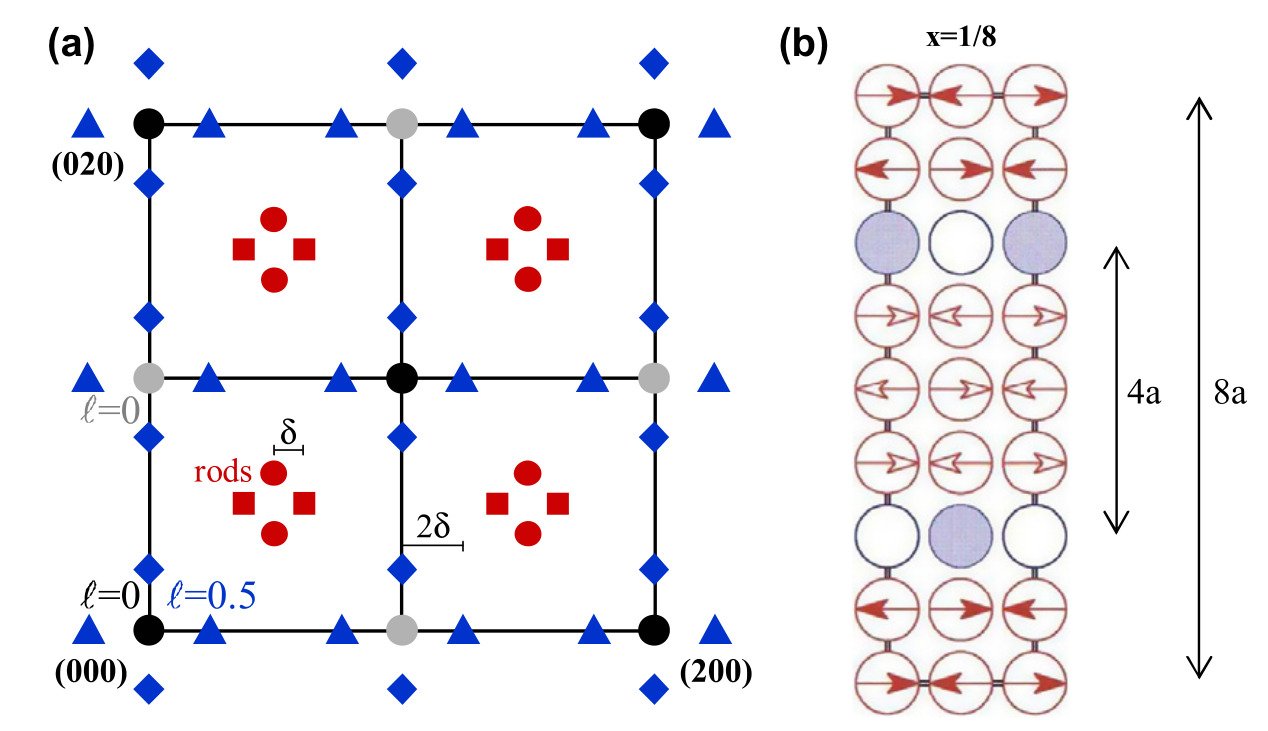
\includegraphics[width=0.8\textwidth]{fig/intro/stripe_model_hucker.png}
    \caption[stripe model hucker]{stripe model hucker \cite{Hucker2012}}
    \label{fig:stripe_model_hucker}
\end{figure}

This model is appealing because it suggests that superconducting electrons are locally segregated from the localized magnetic electrons. it also seems like a reasonable way to relieve the frustration in the traffic jam analogy (figure \ref{fig:electron_traffic_jam}). When discussing stripes, a distinction between spin stripes and charge stripes is typically made. While evidence mostly points to a picture where charge and spin stripes are simultaneous, charge stripes are much harder to detect and only seem to be associated with the $n_\text{h} = \frac{1}{8}$ phase \cite{Christensen2014, Croft2014,Thampy2014} where spin stripe order is seen in a large part of the phase diagram $0.02 < n_\text{h} < 0.13$ \cite{Julien2003}.

The excitations associated with the spin stripes exhibit the universal hourglass dispersion as we saw in figure \ref{fig:yamada_plot} \cite{Tranquada2004a} and the relationship between stripe order and the associated excitations have been extensively studied as summarized by figure \ref{fig:kofu_phase}. In short, the ordering temperature of spin stripe order increases with doping up to $n_\text{h} \approx \frac{1}{8}$ where the excitations become gapped. In the optimally doped region of the phase diagram, the size of the gap $E_\text{g}$ is roughly of the order $k_\text{B} T_\text{c}$, suggesting a direct connection between the magnetic excitation spectrum and superconductivity.

\begin{figure}
    \centering
    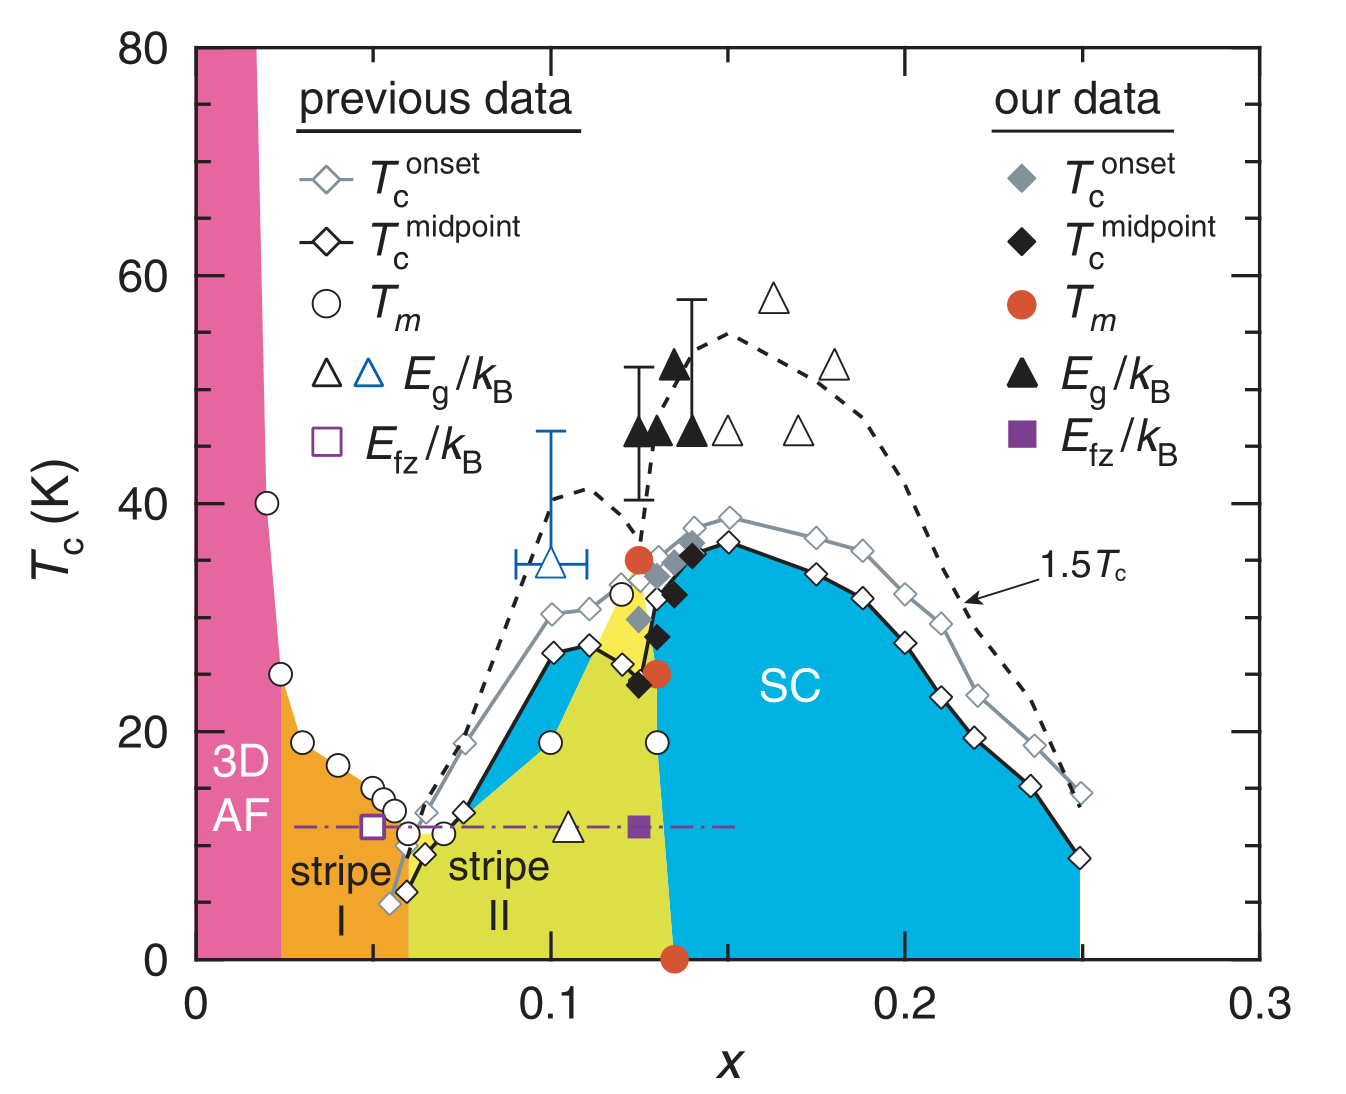
\includegraphics[width=0.6\textwidth]{fig/intro/kofu_phase.png}
    \caption[kofu phase diagram]{kofu phase diagram \cite{Kofu2009}}
    \label{fig:kofu_phase}
\end{figure}

\section{LSCO+O}\label{sec:lscoo}
Finally, we turn to the material studied in this thesis, La$_{2-x}$Sr$_x$CuO$_{4+\delta}$. In addition to the substitutional doping outlined above, La$_2$CuO$_4$ can be doped with additional oxygen using electrochemical methods \cite{Blakeslee1998}, yielding La$_2$CuO$_{4+\delta}$ (LCO+O). These materials are sometimes called over-stoichiometric or super-oxygenated and the additional oxygen can be combined with Sr-doping yielding the so-called `co-doped' samples  LSCO+O. Due to the electrochemical method of introducing the additional oxygen, it can difficult to control the amount of nominal doping, and we are often forced to use relatively imprecise or destructive methods such as titration (see e.g. MSc thesis by Mariam Ahmad in our group) or Thermogravitometric Analysis (TGA) in order to determine the doping $n_\text{h}$.

With that in mind, a comparison of LSCO and LCO+O is sketched in figure \ref{fig:phase_wells}. A peculiar feature of doping with oxygen is the fact that only certain superconducting phases seem to emerge ($T_\text{c} \approx 15, 30, \SI{40}{\kelvin}$) and the amount of each phase can be tuned with oxygen content \cite{Liu2005}, pressure \cite{Lorenz2002} or thermal treatment \cite{Fratini2010}. The white parts of the LCO+O phase diagram is the `miscibility gap', where phases co-exist. I emphasize here that LSCO+O has a slightly better $T_\text{c}$ when compared to LSCO.

\begin{figure}
    \centering
    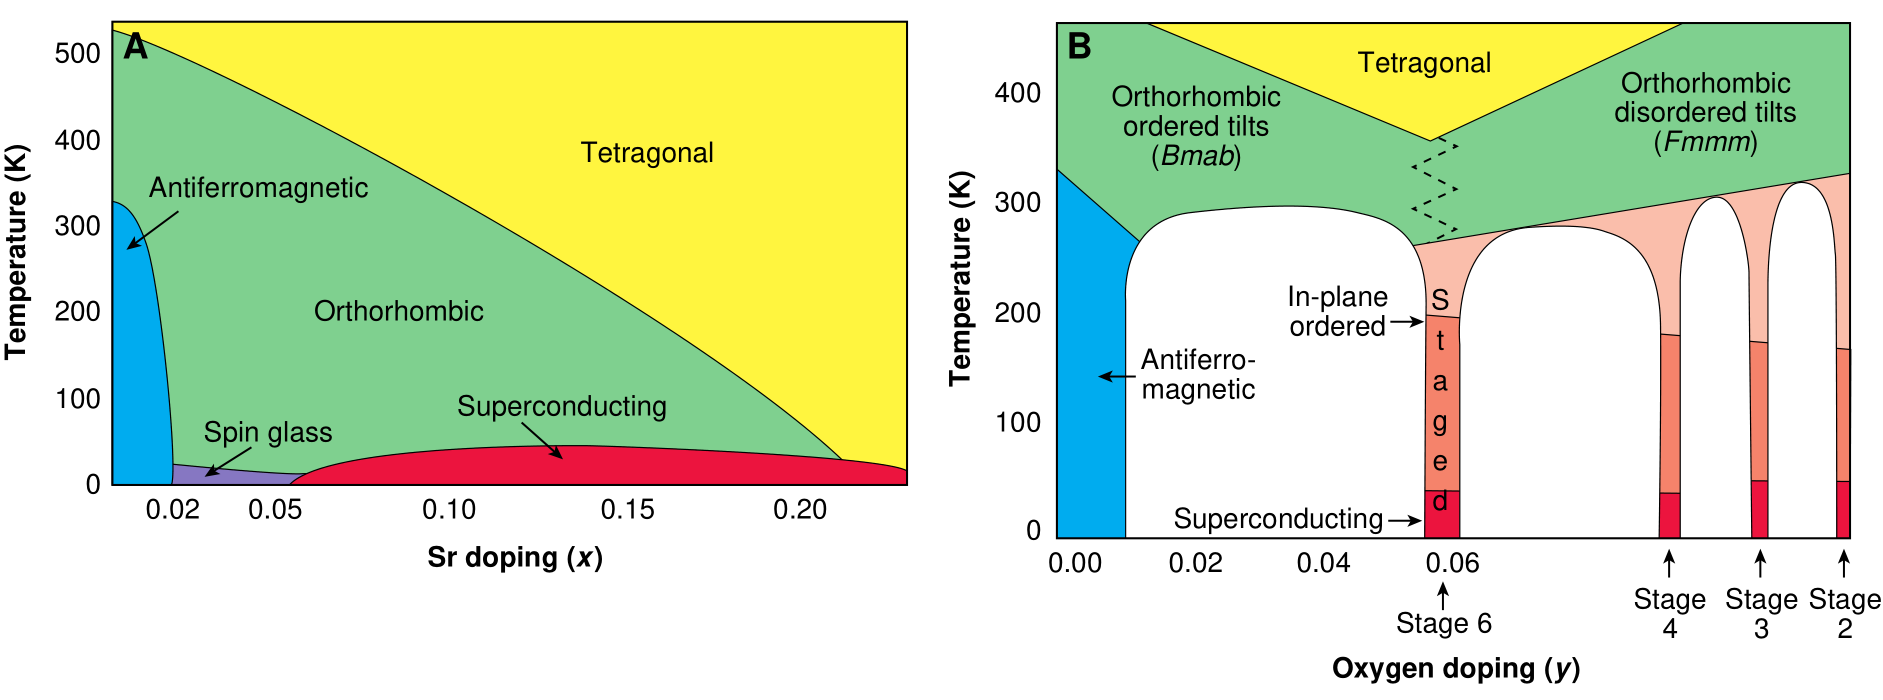
\includegraphics[width=\textwidth]{fig/intro/phases_wells.png}
    \caption[lsco lcoo comparison]{lsco lcoo comparison \cite{Wells1997}}
    \label{fig:phase_wells}
\end{figure}

Since the electrochemical doping procedure essentially pushes oxygen atoms into the lattice, we know that the oxygen is equipped with some level of mobility within the lattice and this mobility is likely the reason for this `discretization' of $T_\text{c}$. Another way of thinking about this is in terms of an `annealed disorder' \cite{Wells1997}, where the oxygen can achieve an optimal inhomogeneity \cite{Poccia2012}. This is in contrast to the `quenched disorder' \cite{Wells1997} of LSCO where the positions of Sr ions are fixed during the solid state synthesis at elevated temperatures ($T \approx \SI{1000}{\celsius}$). 

This annealed disorder results in a number of structural phenomena. First, a structural correlation along the $c$-axis known as staging \cite{Wells1996}, shown in figure \ref{fig:staging}, is likely the result of the lattice trying to accommodate the interstitial oxygens. There is little reason to believe that staging has anything to do with superconductivity since it appears in a very similar way in the isostructural non-superconducting nickelate La$_2$NiO$_4+\delta$ \cite{Tranquada1994} and no direct relation between the staging details and $T_c$ was found in LSCO+O \cite{ray2017}.

\begin{figure}
    \centering
    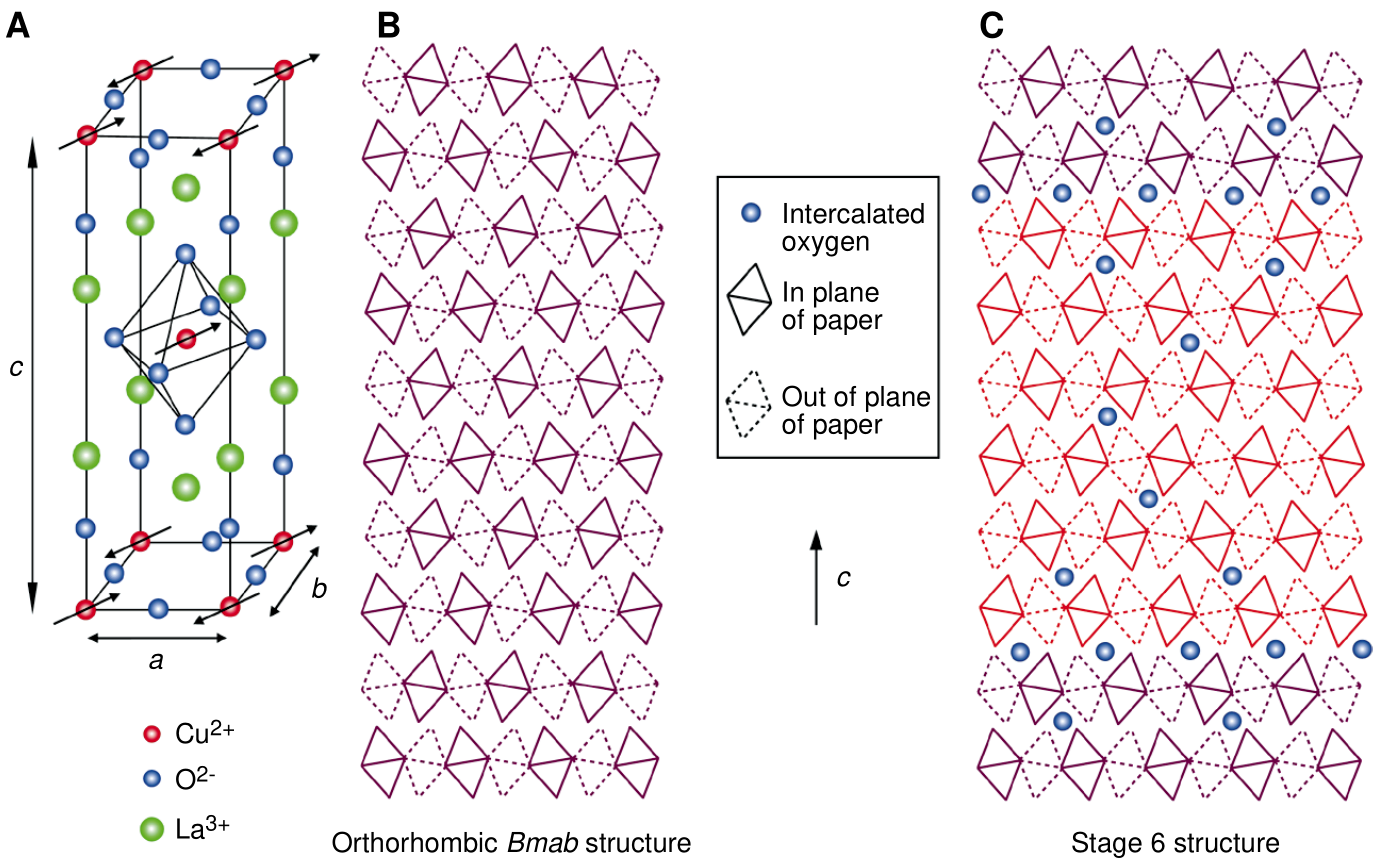
\includegraphics[width=0.6\textwidth]{fig/intro/staging.png}
    \caption[staging]{Illustration of staging in LCO+O, from \cite{Wells1997}. \textbf{A:} Crystal structure of La$_2$CuO$_4$, highlighting the octahedra centred at the copper atom. \textbf{B:} Displacement pattern of these octahedra as viewed from the side. \textbf{C:} Staging pattern due to intercalated oxygen. By creating anti-phase boundaries the structure accommodates the oxygen atoms in an energetically favourable way. The number of CuO$_2$ planes between the anti-phase boundaries determines the staging number (in this case stage-6)}
    \label{fig:staging}
\end{figure}

A more complex three dimensional ordering has been observed both by neutrons \cite{Lee2004, ray} and by x-ray micro-diffraction \cite{Fratini2010, Poccia2012}. Since thermal treatments that modify the superconducting phases simultaneously removes some of these structural features \cite{Poccia2012}, it has been suggested that these superstructures might be related to superconductivity through the `superstripes' idea \cite{Bianconi2000}.

A peculiar feature of LSCO+O, is the fact that the superconducting and magnetic phases of LSCO+O are distinct and separate. Magnetic susceptibility and muon-spin-rotation ($\mu$SR) measurements have revealed a linear relationship between the volumes of the two phases, suggesting that they are separated in real space \cite{Mohottala2006,Udby2013}. In the context of the LSCO phase diagram, it is believed that these two phases is one with exactly $n_\text{h} = \frac{1}{8}$ (magnetic) and one with $n_\text{h} \approx 0.16$ (optimally superconducting). Whether this phase separation is unique to LSCO+O is hard to say -- one could imagine a scenario where the annealed doping of LSCO+O allows these phases to `grow' in contrast to LSCO with only quenched doping from Sr \cite{Udby2013}.

Finally, LSCO+O (with one exception, see chapter \ref{ch:anomaly}) is equipped with static stripe order despite having a $T_\text{c}$ reminiscent of optimally doped LSCO. In addition, the transition temperature of this static order $T_\text{N}$ coincides with $T_\text{c}$ \cite{Udby2013}, suggesting a unique and direct connection between the two electronic phases in this compound.

LSCO+O is thus structurally and electronically distinct from LSCO, while still exhibiting the universal features of the cuprates in a consistent way. This system is important in the larger context because, as we learned in this chapter, 1) the cuprates are fundamentally inhomogeneous systems and 2) the fact that crystal structure clearly interacts with the superconducting state and/or stripe order. Since LSCO+O is unique on these two counts, an investigation of this system can help us understand those unsolved issues.

\section{Thesis objectives}
The objective of this thesis is to investigate phonon dynamics of the LSCO+O system through neutron scattering measurements and molecular simulations. The idea is to consider here the full three dimensional lattice of the cuprates by trying to understand how the surrounding lattice interacts with the CuO$_2$ planes (which are usually studied). The strategy is to primarily focus on the dynamical aspects of the lattice by measuring and simulating phonons in the system. While phonon-mediated superconductivity in the manner of conventional BCS theory is unlikely in the cuprates, a better understanding of the lattice dynamical effects in the cuprates, and possibly indrect effects on superconductivity could be useful to the community as a whole.

In this context I will mention a few experimental result that emphasizes this motivation. Recently, a longitudinal study of several different cuprates suggested that the Cu-O distance to the apical oxygen (the oxygen atoms directly above and below the copper atoms) has an effect on the in-plane exchange interaction \cite{Peng2017}. A different study on thin films showed a similar effect on the in-plane Cu-O distances \cite{Ivashko2019}. Finally, a measurement of atomic pair distribution functions as a function of doping in LSCO has shown that the \emph{distribution} of in-plane Cu-O distances is broadest at optimal doping, suggesting that a phase separation picture might be relevant for LSCO.

Just as with stripes picture, the excitations are just as relevant as the static order. In the same way, a study of phonons might reveal subtleties that we have not been able to discern from a purely structural viewpoint. The goal of this thesis is thus to carefully evaluate the phonon spectrum of LCO, LSCO, LCO+O and LSCO+O in theory and practice. This is done with various techniques in neutron scattering and simulations with density functional theory. In a more concrete way, the problem statement of this thesis is:

\begin{quote}
    \todo{insert brilliant problem statement.}
\end{quote}

\subsection{Outline}
\todo{write outline when chapters are done.}
